\documentclass{article}[18pt]
\usepackage{../../../../../format}
\lhead{MCS - LDS}


\begin{document}
\begin{center}
\underline{\huge Discrete Structures - Relations}
\end{center}
\section{Binary relations}
Let A and B be sets. A \textbf{binary relation R from A to B} is a subset of the cartesian product $A\times B$\\
(Or, equivalently, a binary relation R is a set of ordered pairs
where the first element comes from A and the second element
from B.)
\begin{itemize}
	\item We write $(a,b)\in R$ or say that $R(a,b)$ \textbf{holds} if the ordered pair (a,b) is in the binary relation R
	\item We write $(a,b)\notin R$ or say that $R(a,b)$ \textbf{does not hold} or say that $\lnot R(a,b)$ \textbf{holds} if the ordered pair $(a,b)$ is not in R
\end{itemize}
\section{Functions as binary relations}
\textbf{Functions} can be viewed as binary relations.\\
If $f:A\rightarrow B$ then the graph of the function f is the binary relation $\{ ( a , f ( a ) ) : a \in A \} \subseteq A \times B$\\
Conversely, not every binary relation R from A to B can be considered to be the graph of a function:
\begin{itemize}
	\item we need R to have the property that every element a of A appears in (as the first component) \textbf{exactly} 1 element (a,b) of R
	\item if this is so then the corresponding function f is defined as $f(a)=$ the unique element $b\in B$ for which $(a,b)\in R$
\end{itemize}
In general, binary relations are generalizations of functions and can be used to describe a much wider class of relationships
\section{Relations on a set}
We can have \textbf{relations} involving \textbf{more} than two sets; that is, relations that are subsets of the Cartesian product of any number of sets.\\
If a relation R is a subset of $A _ { 1 } \times A _ { 2 } \times \cdots \times A _ { n } ,$ for some $n \geq 1$ then we say that R has an arity n or is n-ary relation\\
Henceforth, we simply refer to all relations as simply 'relations' and only add terms such as 'binary' or 'n-ary' when required.\\
The \textbf{binary relation R on a set A} is a relation from A to A; that is, a subset of $A\times A$\\
\\
We can also have n-ary relations on sets; that is, subsets of $A\times A\times \cdots \times A$ (repeated n times)
\section{Properties of relations}
\subsection{Reflexive}
A binary relation R on A is \textbf{reflexive} if $( a , a ) \in R , \forall a \in A$\\
\\
A relation R on A of arity greater than 2 can also be reflexive, we insist that $( a , a , \dots , a ) \in R , \forall a \in A$
\subsection{Irreflexive}
A binary relation R on A is irreflexive if $( a , a ) \notin R , \forall a \in A$\\
\\
A relation R on A of arity greater than 2 can also be irreflexive: we insist that $( a , a , \ldots , a ) \notin R , \forall a \in A$
\subsection{Symmetry and anti-symmetry}
A binary relation R on A is symmetric if:
$$( a , b ) \in R , \text { then } ( b , a ) \in R \forall a , b \in A$$
A binary relation R on A is anti-symmetric if:
$$( a , b ) , ( b , a ) \in R , \text { then } a = b \forall a , b \in A$$
(or we do not have $( a , b ) , ( b , a ) \in R$ if $a \neq b$ )
\subsection{Transitivity}
A binary relation R on A is \textbf{transitive} if:
$$( a , b ) , ( b , c ) \in R \text { then } ( a , c ) \in R , \forall a , b , c \in A$$
\section{Combining Relations}
As relations are just sets (of tuples), all operations that can be applied to sets can be applied to relations.\\
Also, just as functions can be \textbf{composed}, so can relations\\
Let $R \subseteq A \times B$ and $S \subseteq B \times C$ be relations. The \textbf{composite relation} $S \circ R \subseteq A \times C$ is defined as:
$$\{ ( a , c ) : a \in A , c \in C , \exists b \in B \text { s.t. } ( a , b ) \in R \text { and } ( b , c ) \in S \}$$
\section{Composing a relation with itself}
Suppose that $R\subseteq A\times A$ We can \textbf{compose R with itself} so that
$$R \circ R = \{ ( a , c ) : a , c \in A , \exists b \in A \text { s.t. } ( a , b ) , ( b , c ) \in R \}$$
We denote $R\circ R$ by $R^2$\\
In general, we denote $R \circ R \circ \cdots \circ R$ (repeated n times) by $R^n$ (with $R^0$ and $\varnothing$ and $R^1$ defined as R)\\
Note that it does not matter the order we choose to build $R^n$. For example, $R\circ (R\circ R)$ is the same relation as $(R\circ R)\circ R$
\begin{itemize}
	\item As an illustration, suppose that we have a \textbf{directed graph} G with vertex set V and edge set E. The edge set is a relation $E\subseteq V\times V$
\end{itemize}
\section{Projections}
Suppose that we have some n-ary relation R such that
$$R \subseteq A _ { 1 } \times A _ { 2 } \times \cdots \times A _ { n }$$
We can build a new m-cry relation from R, where $m<n$, by projecting
\begin{itemize}
	\item Choose $i_1,i_2,...,i_m\in \{1,2,...,n\}$, where $i_1<i_2<..<i_m$
	\item Build the m-ary relation $S \subseteq A _ { i _ { 1 } } \times A _ { i _ { 2 } } \times \cdots \times A _ { i_m }$ by taking all those m-tuples that are obtained from some n-tuple of R bu only including the elements in components $i_1,i_2,...,i_m$
	\item The relation S is the \textbf{projection} of R in components $i_1,i_2,...,i_m$
\end{itemize}
\section{Closures of relations}
Let $R\subseteq A\times A$\\
The \textbf{reflexive closure} of R is the smallest reflexive relation that contains R. It is obtained by adding to R all the pair (x,x) that do not already lie in R\\
The \textbf{symmetric closure} of R is the smallest symmetric relation that contains R. It is obtained by adding to R all the pairs(x,y) for which (y,x) (but not (x,y)) lies in R\\
The \textbf{transitive closure} of R is the smallest transitive relation that contains R. It is the relation defined as
$$\left\{ ( a , b ) : a , b \in A , ( a , b ) \in R ^ { n } , \text { for some } n \geq 1 \right\} = \bigcup _ { n = 1 } ^ { \infty } R ^ { n }$$
\section{Equivalence Relations}
A relation $R\subseteq A\times A$ is called an \textbf{equivalence relation} if it is \textbf{reflexive, symmetric and transitive}\\
If R is an equivalence relation and $(a,b)\in R$ then a and b are \textbf{equivalent} and we sometimes write $a\equiv b$ or $a\sim b$ (note that $b\equiv a$ also)\\
Let $a\in A$. The \textbf{equivalence class} containing a, written as $[a]_R$ is the set of all elements z that are equivalent to a.\\
Note that all elements in $[a]_R$ are equivalent to each other\\
So, if $x\in [a]_R$ then $a\in [x]_R$ and $[a]_R=[x]_R$\\
In particular, no element of a can be in two different equivalence classes; that is, if $[a]_R\neq [b]_R$ then $[a]_R\cap [b]_R=\varnothing$\\
So the distinct equivalence classes of R partition A; that is, A can be written as the disjoint union of equivalence classes.
\section{Partial orders}
A binary relation that is reflexive, anti symmetric and transitive is called a partial order.\\
A set S together with a partial order R on S is called a partially ordered set (or \textbf{poset}) and written (S,R).\\
\\
We often denote the partial order relation in a poset by $\leqslant$ even though we way not be referring to the usual ordering on numbers, and write $a\leqslant b$ rather than $\leqslant (a,b)$\\
If $(S,\leqslant)$ is some poset then two elements of S are comparable if either $a\leqslant b$ or $b\leqslant a$, and incomparable otherwise
\section{Using posets in communication protocols}
Suppose that we have two devices, A and B, sending messages to one another according to some protocol.\\
A \textbf{trace} of this system is a sequence of messages where each message comes with:
\begin{itemize}
	\item the time it was sent and the time it was received
\end{itemize} 
However, the two device clocks are not synchronised and might run at different speeds:
\begin{itemize}
	\item so a time on device A cannot be compared with a time on device B
\end{itemize}
The delivery of a message takes a non-zero amount of time. A typical trace might be (with events in increasing time order)
\begin{itemize}
	\item device A: send $m_1$; receive $m_2$; send $m_3$, receive $m_4$
	\item device B: send $m_2$; receive $m_1$; send $m_4$; receive $m_3$
\end{itemize}
We can think of our example trace as a relation R on a set E
 $$\begin{array} { l } { E = \left\{ s _ { 1 } , r _ { 1 } , s _ { 2 } , r _ { 2 } , s _ { 3 } , r _ { 3 } , s _ { 4 } , r _ { 4 } \right\} } \\ { R = \left\{ \left( s _ { 1 } , r _ { 1 } \right) , \left( s _ { 2 } , r _ { 2 } \right) , \left( s _ { 3 } , r _ { 3 } \right) , \left( s _ { 4 } , r _ { 4 } \right) , \left( s _ { 1 } , r _ { 2 } \right) \right. } \\ { \quad \left( r _ { 2 } , s _ { 3 } \right) , \left( s _ { 3 } , r _ { 4 } \right) , \left( s _ { 2 } , r _ { 1 } \right) , \left( r _ { 1 } , s _ { 4 } \right) , \left( s _ { 4 } , r _ { 3 } \right) \} } \end{array}$$
 \begin{center}
 	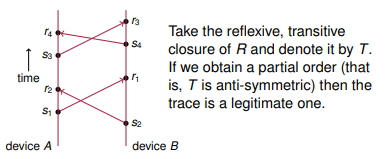
\includegraphics[scale=0.7]{coms}
 \end{center}
 \section{Total and well orders}
 If $(S,\leqslant)$ is a poset, and further, every two elements in S are comparable then S is a \textbf{totally ordered set} or \textbf{linearly ordered set}, with $\leqslant$ a \textbf{total ordering} or \textbf{linear ordering}
\begin{itemize}
 	\item The poset $(\mathbb{Z},\leqslant)$ is totally ordered (as $a\leqslant b$ or $b\leqslant a$ $\forall a,b \in \mathbb{Z}$)
\end{itemize}
If $(S,\leqslant)$ is a poset and, further, $\leqslant$ is a total ordering and every non empty subset of S has a least element (under $\leqslant$) then $(S,\leqslant)$ is a \textbf{well-ordered set}.
\section{Lexicographic orders}
If $(A,\leqslant_A)$ and $(B,\leqslant_B)$ are two posets then define the lexicographic ordering $\leqslant$ on $A\times B$  by $(a,b)\leqslant(a',b')$ if and only f
\begin{itemize}
	\item $a\leqslant_A a'$ and $a\neq a'$, or
	\item $a=a'$ and $b\leqslant_B b'$
\end{itemize}
With $(a,b)=(a',b')$ if and only if $a=a'$ and $b=b'$\\
$(A\times B,\leqslant)$ is a poset.\\
\\
Lexicographic orders can be extended to more than two posets.\\
Let $(A_j,\leqslant_i)$ be a poset, for i=1,2,...,n. Consider the cartesian product $A_1\times A_2\times...\times A_n$, where $n\geqslant 2$. We say that $(a_1,a_2,...,a_n)\leqslant (b_1,b_2,...,b_n)$ in the lexicographic order $\leqslant$ on $A_1\times A_2 \times ... \times A_n$ if and only if
\begin{itemize}
	\item $a_1=b_1, a_2=b_2,...,a_n=b_n$ or
	\item $\exists j\in \{1,2,...,n\}$ such that ( A , \textbackslash\{\}leq A ) $a _ { 1 } = b _ { 1 } , a _ { 2 } = b _ { 2 } , \dots , a _ { j - 1 } = b _ { j - 1 } , a _ { j } \leq_j b _ { j } , a _ { j } \neq b _ { j }$
\end{itemize}

\end{document} 